\documentclass{article}
\usepackage[margin=1in]{geometry}
\usepackage{hyperref}
\usepackage{tikz}
\usetikzlibrary{positioning, shapes.geometric}

\title{Cryptography and Network Security\\Practical 1}
\author{DevParapalli}
\date{2024-08-07}

\begin{document}

\maketitle

\section{Cryptography}

Cryptography is the science of secure communication in the presence of adversaries. It encompasses techniques for ensuring confidentiality, integrity, authentication, and non-repudiation of information. The word "cryptography" comes from the Greek words "kryptos," meaning hidden, and "graphein," meaning to write. In essence, cryptography is about constructing and analyzing protocols that prevent third parties or the public from reading private messages.

In the digital age, cryptography has become an essential tool for protecting sensitive information in various domains, including finance, healthcare, government, and personal communications. It forms the backbone of many security protocols and is fundamental to the functioning of secure systems on the internet. As cyber threats continue to evolve, the importance of robust cryptographic systems cannot be overstated.

\section{Principles of Cryptography}

The core principles of cryptography revolve around four main objectives: confidentiality, integrity, authentication, and non-repudiation. Confidentiality ensures that information is kept secret from unauthorized parties. This is typically achieved through encryption, where plaintext is converted into ciphertext using a cryptographic algorithm and a key. Integrity guarantees that the information has not been altered during transmission or storage. This is often implemented using cryptographic hash functions and digital signatures.

Authentication verifies the identity of the parties involved in a communication, ensuring that the sender is who they claim to be. This is crucial in preventing impersonation attacks and is commonly implemented using digital certificates and public key infrastructure (PKI). Non-repudiation provides proof of the origin of information, preventing a sender from denying they sent a message. This principle is particularly important in legal and financial contexts and is typically achieved through the use of digital signatures and trusted third parties.

\section{Diagram \& Explanation}

\begin{figure}[h]
    \centering
    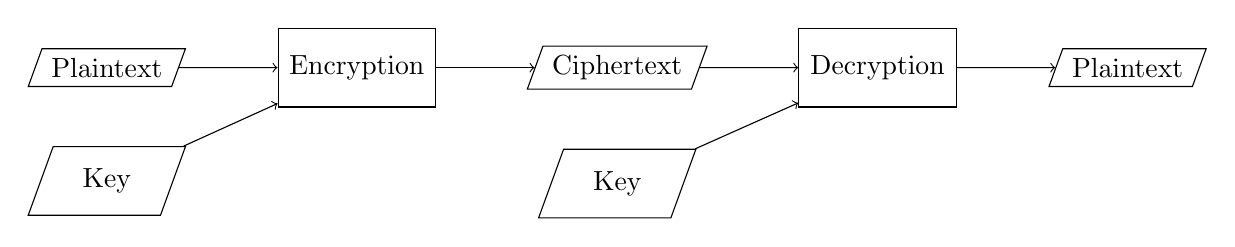
\begin{tikzpicture}[
        node distance = .75cm and 1.25cm,
        box/.style = {rectangle, draw, minimum width=2cm, minimum height=1cm},
        io/.style = {trapezium, trapezium left angle=70, trapezium right angle=110, draw, minimum width=2cm}
    ]
        % Encryption process
        \node[io] (plaintext1) {Plaintext};
        \node[io, below=of plaintext1] (enckey) {Key};
        \node[box, right=of plaintext1] (enc) {Encryption};
        \node[io, right=of enc] (ciphertext) {Ciphertext};
        
        % Decryption process
        \node[io, below=of ciphertext] (deckey) {Key};
        \node[box, right=of ciphertext] (dec) {Decryption};
        \node[io, right=of dec] (plaintext2) {Plaintext};
        
        % Arrows
        \draw[->] (plaintext1) -- (enc);
        \draw[->] (enckey) -- (enc);
        \draw[->] (enc) -- (ciphertext);
        \draw[->] (ciphertext) -- (dec);
        \draw[->] (deckey) -- (dec);
        \draw[->] (dec) -- (plaintext2);
    \end{tikzpicture}
    \caption{Encryption and Decryption Process}
    \end{figure}

The diagram above illustrates the basic process of encryption and decryption in cryptography. The process begins with plaintext, which is the original, readable message. This plaintext is then transformed into ciphertext using an encryption algorithm and an encryption key. The ciphertext is the scrambled, unreadable version of the message that can be safely transmitted or stored. To recover the original message, the recipient uses a decryption algorithm along with the appropriate decryption key to convert the ciphertext back into plaintext.

In symmetric key cryptography, the same key is used for both encryption and decryption. This method is fast but requires secure key exchange. In asymmetric or public key cryptography, different keys are used for encryption and decryption. This solves the key distribution problem but is computationally more intensive. Modern cryptographic systems often use a combination of both approaches to leverage their respective strengths.

\section{Importance of Cryptography}

The importance of cryptography in today's digital world cannot be overstated. It plays a crucial role in protecting sensitive information, securing communications, and enabling trust in digital transactions. In the realm of e-commerce, cryptography ensures that financial transactions are secure, protecting credit card numbers and personal financial information from interception and misuse. In the healthcare sector, it safeguards patient records, ensuring compliance with privacy regulations such as HIPAA.

Cryptography is also fundamental to national security, protecting classified information and secure communications between government agencies and military personnel. In the corporate world, it helps protect trade secrets and intellectual property. On a personal level, cryptography secures our daily digital interactions, from messaging apps to email communications. As our reliance on digital technologies continues to grow, so does the importance of robust cryptographic systems in maintaining privacy, security, and trust in the digital ecosystem.

\section{Cryptography Attack Types}

Cryptographic attacks are attempts to circumvent the security provided by cryptographic systems. These attacks can be broadly categorized into cryptanalytic attacks and implementation attacks. Cryptanalytic attacks focus on finding weaknesses in the mathematical algorithms underlying cryptographic systems. Some common types include:

\begin{enumerate}
    \item Brute Force Attack: This involves trying every possible key until the correct one is found.
    \item Frequency Analysis: Used against simple substitution ciphers, this attack exploits the frequency distribution of letters in a language.
    \item Man-in-the-Middle Attack: The attacker intercepts communications between two parties, potentially altering the messages.
    \item Known Plaintext Attack: The attacker has access to both the plaintext and its encrypted version and uses this to deduce the key.
\end{enumerate}

Implementation attacks, on the other hand, target weaknesses in the implementation of cryptographic systems rather than the algorithms themselves. These include:

\begin{enumerate}
    \item Side-Channel Attacks: These exploit information leaked by the physical implementation of a cryptosystem, such as power consumption or electromagnetic emissions.
    \item Timing Attacks: The attacker analyzes the time taken to execute cryptographic algorithms to deduce secret information.
    \item Fault Injection: This involves introducing faults into a cryptographic system to cause it to produce incorrect results, which can then be analyzed to deduce secret information.
\end{enumerate}

Understanding these attack types is crucial for designing robust cryptographic systems and implementing appropriate countermeasures.

\section{Network Security}

Network security encompasses the policies, practices, and technologies employed to protect network infrastructure, data, and users from unauthorized access, misuse, modification, or denial of service. It involves a multi-layered approach that addresses both the hardware and software aspects of network systems. The goal of network security is to maintain the confidentiality, integrity, and availability of network resources and information.

In today's interconnected world, where organizations rely heavily on network-based systems for their operations, effective network security is more critical than ever. It protects against a wide range of threats, including malware, hacking attempts, data breaches, and insider threats. Network security also plays a crucial role in ensuring compliance with various regulatory requirements, such as GDPR, HIPAA, and PCI DSS, which mandate the protection of sensitive data.

\section{Network Security Model}

A comprehensive network security model typically follows a defense-in-depth approach, implementing multiple layers of security controls. This model can be conceptualized as concentric rings of protection, with each layer focusing on specific aspects of security. The layers in a typical network security model include:

\begin{enumerate}
    \item Perimeter Security: This outermost layer includes firewalls, intrusion detection/prevention systems (IDS/IPS), and virtual private networks (VPNs) to control incoming and outgoing network traffic.
    \item Network Security: This layer focuses on securing the internal network infrastructure, including network segmentation, access controls, and secure protocols.
    \item Host Security: At this level, individual devices are secured through measures such as antivirus software, host-based firewalls, and patch management.
    \item Application Security: This layer addresses security at the application level, including secure coding practices, input validation, and authentication mechanisms.
    \item Data Security: The innermost layer focuses on protecting the data itself through encryption, access controls, and data loss prevention (DLP) technologies.
\end{enumerate}

This layered approach ensures that if one security measure fails, others are in place to detect and mitigate threats, providing a more robust overall security posture.

\section{Security Attacks}

Security attacks in the context of network security can be broadly categorized into passive and active attacks. Passive attacks involve the unauthorized interception of information without altering it. These attacks are difficult to detect as they do not involve any modification of data. Examples include eavesdropping and traffic analysis. Active attacks, on the other hand, involve the modification of data or the creation of false data streams. These are generally easier to detect but can cause significant damage. Examples of active attacks include:

\begin{enumerate}
    \item Denial of Service (DoS) and Distributed Denial of Service (DDoS) attacks: These aim to make network resources unavailable to legitimate users.
    \item Man-in-the-Middle (MitM) attacks: The attacker intercepts and potentially alters communication between two parties.
    \item SQL Injection: This attack targets vulnerabilities in database-driven applications to manipulate or retrieve data.
    \item Cross-Site Scripting (XSS): This involves injecting malicious scripts into web pages viewed by other users.
\end{enumerate}

Understanding the nature and mechanics of these attacks is crucial for developing effective defense strategies and implementing appropriate security measures.

\section{Importance of Network Security}

The importance of network security in today's digital landscape cannot be overstated. As organizations increasingly rely on digital infrastructure for their operations, the potential impact of security breaches has grown exponentially. Effective network security is crucial for several reasons:

\begin{enumerate}
    \item Protection of Sensitive Data: Network security safeguards confidential information such as financial data, personal information, and intellectual property from unauthorized access and theft.
    \item Maintaining Business Continuity: By preventing and mitigating attacks, network security helps ensure that business operations can continue without disruption.
    \item Compliance with Regulations: Many industries are subject to strict data protection regulations. Network security helps organizations meet these compliance requirements and avoid potential legal and financial penalties.
    \item Preserving Reputation: Security breaches can severely damage an organization's reputation, leading to loss of customer trust and business opportunities. Strong network security helps maintain stakeholder confidence.
\end{enumerate}

Moreover, as cyber threats continue to evolve in sophistication and scale, the importance of robust network security measures becomes even more critical. Organizations must continuously adapt and improve their security posture to stay ahead of emerging threats and protect their digital assets effectively.

\section{Application of Network Security}

Network security finds application across various domains and industries, each with its unique requirements and challenges. Some key areas of application include:

\begin{enumerate}
    \item Enterprise Networks: Large organizations implement comprehensive network security solutions to protect their corporate networks, which often span multiple locations and include remote access capabilities.
    \item E-commerce Platforms: Online retailers and financial institutions rely heavily on network security to protect customer data and financial transactions.
    \item Healthcare Systems: The healthcare industry requires robust network security to protect patient data and comply with regulations like HIPAA.
    \item Government and Military Networks: These sectors require the highest levels of security to protect classified information and critical infrastructure.
    \item Internet of Things (IoT) Networks: As IoT devices proliferate, securing these networks becomes crucial to prevent unauthorized access and potential exploitation.
\end{enumerate}

The application of network security often involves a combination of technologies such as firewalls, intrusion detection systems, virtual private networks (VPNs), and encryption protocols. It also encompasses practices like regular security audits, employee training, and incident response planning. As the threat landscape evolves, so do the applications of network security, with emerging technologies like artificial intelligence and machine learning being increasingly used to enhance threat detection and response capabilities.

\section{Conclusion}

In conclusion, cryptography and network security are fundamental pillars of our digital infrastructure, playing crucial roles in protecting sensitive information, enabling secure communications, and maintaining the integrity of digital systems.

\end{document}